% --- ANNEXES ---
\appendix
\part*{Annexes}
\addcontentsline{toc}{part}{Annexes}

\chapter{Corpus du benchmark RAG et vérité-terrain}
\label{annexe:corpus}

Cette annexe rassemble le corpus complet des 30 questions métier du benchmark comparatif RAG cloud/local (section~\ref{chap:benchmark_rag}, §\ref{sec:bench_protocole}) sa vérité-terrain et le verdict attribué à chaque réponse, à des fins de reproductibilité. Le corpus et les résultats bruts sont versionnés dans le dépôt \texttt{assistant-soyaff-1} (\texttt{benchmark/questions.csv} ; \texttt{benchmark/resultats/vps\_20260927\_2143/}, qui contient les réponses brutes, la vérité-terrain recalculée sur la base de production et l'état du système avant et après la mesure). Ces fichiers font foi en cas d'écart avec les tableaux qui suivent.

\section{Les 30 questions, par catégorie et type de vérité-terrain}

\begin{longtable}{|>{\raggedright\arraybackslash}p{0.9cm}|>{\raggedright\arraybackslash}p{2.7cm}|>{\raggedright\arraybackslash}p{0.9cm}|>{\raggedright\arraybackslash}p{9.2cm}|}
\caption{Corpus des 30 questions métier du benchmark}
\label{tab:annexe_corpus} \\
\hline
\rowcolor[HTML]{EFEFEF}
\textbf{ID} & \textbf{Catégorie} & \textbf{Type} & \textbf{Question} \\ \hline
\endfirsthead
\multicolumn{4}{c}{\tablename\ \thetable\ (suite)} \\ \hline
\rowcolor[HTML]{EFEFEF}
\textbf{ID} & \textbf{Catégorie} & \textbf{Type} & \textbf{Question} \\ \hline
\endhead
Q01 & suivi de flotte & T1 & Combien de camions de type « particulier » ont eu au moins une transaction enregistrée en mars 2026 ? \\ \hline
Q02 & suivi de flotte & T1 & Combien de camions sont actuellement enregistrés avec le statut « actif » dans le système ? \\ \hline
Q03 & suivi de flotte & T2 & Quels camions sont actuellement en statut « maintenance » ? \\ \hline
Q04 & suivi de flotte & T1 & Combien de camions immatriculés au Mali sont des camions de la société (hors particuliers) ? \\ \hline
Q05 & suivi de flotte & T2 & Quels camions n'ont jamais eu de transaction enregistrée depuis leur création ? \\ \hline
Q06 & suivi de flotte & T3 & Comment se répartit la flotte entre camions société et camions particuliers selon le pays d'immatriculation, et que révèle cette répartition sur la structure logistique de SOYAFF ? \\ \hline
Q07 & gestion financière & T1 & Quel est le total des dépenses de carburant du camion CA~0043~MD, toutes périodes confondues ? \\ \hline
Q08 & gestion financière & T1 & Quel est le montant total des amendes enregistrées en mars 2026, tous camions confondus ? \\ \hline
Q09 & gestion financière & T2 & Quels sont les trois camions ayant le plus dépensé en maintenance sur toute la période ? \\ \hline
Q10 & gestion financière & T1 & Quel est le montant total des avances transport versées en mai 2025 ? \\ \hline
Q11 & gestion financière & T2 & Quelles catégories de dépenses dépassent 40 millions de FCFA cumulés sur toute la période ? \\ \hline
Q12 & gestion financière & T3 & Comment la structure des dépenses par catégorie a-t-elle évolué, et quelles catégories pèsent le plus sur la trésorerie de SOYAFF ? \\ \hline
Q13 & analyse des incidents & T1 & Combien d'amendes ont été enregistrées au total depuis le début du suivi (juin 2024) ? \\ \hline
Q14 & analyse des incidents & T2 & Quels camions ont eu au moins une amende en mars 2026 ? \\ \hline
Q15 & analyse des incidents & T1 & Quel est le montant total des amendes payées par le camion CA~6092~MD, toutes périodes confondues ? \\ \hline
Q16 & analyse des incidents & T2 & Quels camions ont enregistré plus de 15 amendes sur toute la période ? \\ \hline
Q17 & analyse des incidents & T1 & Combien de camions distincts ont eu au moins une intervention de maintenance sur la période ? \\ \hline
Q18 & analyse des incidents & T3 & Que révèle la répartition des amendes par camion sur les pratiques de conduite ou les zones à risque du corridor Dakar--Bamako ? \\ \hline
Q19 & conformité documentaire & T1 & Combien de bons de livraison ont été émis en mars 2026 ? \\ \hline
Q20 & conformité documentaire & T2 & Quels bons de livraison n'ont aucun produit associé (bons « orphelins ») ? \\ \hline
Q21 & conformité documentaire & T1 & Combien de bons de livraison ont été émis au total depuis le début du suivi ? \\ \hline
Q22 & conformité documentaire & T1 & Combien de bons de livraison sont actuellement au statut « livré » ? \\ \hline
Q23 & conformité documentaire & T2 & Quels bons de livraison sont associés au camion AA~076~AH ? \\ \hline
Q24 & conformité documentaire & T3 & Le fait que la quasi-totalité des bons de livraison restent au statut « en\_cours » révèle-t-il une lacune dans le processus de clôture documentaire ? Quelles recommandations en tirer ? \\ \hline
Q25 & décision stratégique & T1 & Quel est le montant total des dépenses de ration au premier trimestre 2026 ? \\ \hline
Q26 & décision stratégique & T2 & Quels sont les trois trimestres ayant enregistré les dépenses de ration les plus élevées ? \\ \hline
Q27 & décision stratégique & T1 & Quel est le nombre total de transactions enregistrées en mars 2026 ? \\ \hline
Q28 & décision stratégique & T1 & Quel est le montant total des dépenses de chargement sur l'année 2025 ? \\ \hline
Q29 & décision stratégique & T2 & Quelles catégories de dépenses ont dépassé 100 millions de FCFA cumulés sur toute la période ? \\ \hline
Q30 & décision stratégique & T3 & Au vu des tendances de dépenses en carburant et en maintenance sur les deux dernières années, quelle recommandation stratégique feriez-vous à la direction de SOYAFF pour maîtriser les coûts opérationnels du corridor Dakar--Bamako ? \\ \hline
\end{longtable}

\noindent\footnotesize Nom exact de la catégorie en base (\texttt{categorie} de \texttt{questions.csv}) : \texttt{suivi\_flotte}, \texttt{gestion\_financiere}, \texttt{analyse\_incidents}, \texttt{conformite\_documentaire}, \texttt{decision\_strategique}.
\normalsize

\section{Vérité-terrain des questions T1 et T2}

Pour les 25 questions T1/T2, la réponse de référence est le résultat d'une requête SQL en lecture seule, exécutée sur la base de production le 27~septembre~2026, jour de la mesure. Les requêtes sont reproduites ici pour vérification indépendante.

{\footnotesize
\begin{longtable}{|>{\raggedright\arraybackslash}p{0.8cm}|>{\raggedright\arraybackslash}p{4.2cm}|>{\raggedright\arraybackslash}p{8.8cm}|}
\caption{Vérité-terrain SQL des questions T1 et T2 (base de production, 27~septembre~2026)}
\label{tab:annexe_verite_terrain} \\
\hline
\rowcolor[HTML]{EFEFEF}
\textbf{ID} & \textbf{Réponse de référence} & \textbf{Requête SQL} \\ \hline
\endfirsthead
\multicolumn{3}{c}{\tablename\ \thetable\ (suite)} \\ \hline
\rowcolor[HTML]{EFEFEF}
\textbf{ID} & \textbf{Réponse de référence} & \textbf{Requête SQL} \\ \hline
\endhead
Q01 & 24 camions particuliers & \texttt{SELECT COUNT(DISTINCT t.numero\_immatriculation) FROM transactions t JOIN camions c ON t.numero\_immatriculation = c.numero\_immatriculation WHERE c.type\_propriete='particulier' AND t.date\_transaction BETWEEN '2026-03-01' AND '2026-03-31';} \\ \hline
Q02 & 317 camions & \texttt{SELECT COUNT(*) FROM camions WHERE statut='actif';} \\ \hline
Q03 & Aucun camion (liste vide). Question piège : la colonne \texttt{statut} ne contient que la valeur \texttt{'actif'}. & \texttt{SELECT numero\_immatriculation FROM camions WHERE statut='maintenance';} \\ \hline
Q04 & 110 camions & \texttt{SELECT COUNT(*) FROM camions WHERE pays='MALI' AND type\_propriete='camion\_societe';} \\ \hline
Q05 & 9 camions : AA~084~AG, AA~129~JX, AA~540~AZ, AB~543~AZ, AP~8797~MD, AV~3224, CA~60889~MD, CC~6067~MD, CE~1407~MD & \texttt{SELECT numero\_immatriculation FROM camions c WHERE NOT EXISTS (SELECT 1 FROM transactions t WHERE t.numero\_immatriculation = c.numero\_immatriculation) ORDER BY 1;} \\ \hline
Q07 & 856~950 FCFA & \texttt{SELECT SUM(sorties\_depenses) FROM transactions WHERE categorie\_operation='carburant' AND numero\_immatriculation='CA 0043 MD';} \\ \hline
Q08 & 2~517~000 FCFA (60 transactions) & \texttt{SELECT SUM(sorties\_depenses) FROM transactions WHERE categorie\_operation='amende' AND date\_transaction BETWEEN '2026-03-01' AND '2026-03-31';} \\ \hline
Q09 & AV~3224~MD (1~539~500 FCFA), AP~8798~MD (1~388~500 FCFA), BX~0963~MD (1~319~500 FCFA) & \texttt{SELECT numero\_immatriculation, SUM(sorties\_depenses) AS total FROM transactions WHERE categorie\_operation='maintenance' AND numero\_immatriculation IS NOT NULL GROUP BY numero\_immatriculation ORDER BY total DESC LIMIT 3;} \\ \hline
Q10 & 61~779~000 FCFA & \texttt{SELECT SUM(sorties\_depenses) FROM transactions WHERE categorie\_operation='avance\_transport' AND date\_transaction BETWEEN '2025-05-01' AND '2025-05-31';} \\ \hline
Q11 & 6 catégories : autre (426~118~720), avance\_transport (423~294~700), carburant (154~482~127), chargement (85~160~000), frais\_route (76~985~000), amende (41~113~900) & \texttt{SELECT categorie\_operation, SUM(sorties\_depenses) AS total FROM transactions GROUP BY categorie\_operation HAVING SUM(sorties\_depenses) > 40000000 ORDER BY total DESC;} \\ \hline
Q13 & 488 amendes & \texttt{SELECT COUNT(*) FROM transactions WHERE categorie\_operation='amende';} \\ \hline
Q14 & 30 camions (liste complète dans \texttt{ground\_truth.csv}) & \texttt{SELECT DISTINCT numero\_immatriculation FROM transactions WHERE categorie\_operation='amende' AND date\_transaction BETWEEN '2026-03-01' AND '2026-03-31' AND numero\_immatriculation IS NOT NULL ORDER BY 1;} \\ \hline
Q15 & 432~000 FCFA (6 amendes) & \texttt{SELECT SUM(sorties\_depenses) FROM transactions WHERE categorie\_operation='amende' AND numero\_immatriculation='CA 6092 MD';} \\ \hline
Q16 & 9 camions : CA~6082~MD (30), AA~073~AH (23), AA~082~AH (22), CA~6081~MD (18), AA~662~AM (18), AA~751~AM (18), CA~6088~MD (17), CA~6782~MD (17), AS~3270~MD (16) & \texttt{SELECT numero\_immatriculation, COUNT(*) AS nb FROM transactions WHERE categorie\_operation='amende' AND numero\_immatriculation IS NOT NULL GROUP BY numero\_immatriculation HAVING COUNT(*) > 15 ORDER BY nb DESC;} \\ \hline
Q17 & 65 camions distincts & \texttt{SELECT COUNT(DISTINCT numero\_immatriculation) FROM transactions WHERE categorie\_operation='maintenance' AND numero\_immatriculation IS NOT NULL;} \\ \hline
Q19 & 65 bons de livraison & \texttt{SELECT COUNT(*) FROM bons\_livraison WHERE date\_emission BETWEEN '2026-03-01' AND '2026-03-31';} \\ \hline
Q20 & 7 bons : CA~6090~MD, CONTENER, SENILIV2501236, SENILIV2506450, SENILIV2517704, SENILIV2518392, TRANSBORDEMENT & \texttt{SELECT bl.numero\_bl FROM bons\_livraison bl WHERE NOT EXISTS (SELECT 1 FROM bon\_livraison\_produits blp WHERE blp.bon\_livraison\_id = bl.id) ORDER BY 1;} \\ \hline
Q21 & 727 bons de livraison & \texttt{SELECT COUNT(*) FROM bons\_livraison;} \\ \hline
Q22 & 0 (aucun). Question piège : tous les bons sont au statut \texttt{'en\_cours'}, aucun \texttt{'livre'} ni \texttt{'annule'}. & \texttt{SELECT COUNT(*) FROM bons\_livraison WHERE statut='livre';} \\ \hline
Q23 & 10 bons distincts (liste complète dans \texttt{ground\_truth.csv}) & \texttt{SELECT DISTINCT bl.numero\_bl FROM bons\_livraison bl JOIN transactions t ON t.bon\_livraison\_id = bl.id WHERE t.numero\_immatriculation = 'AA 076 AH' ORDER BY 1;} \\ \hline
Q25 & 3~260~000 FCFA & \texttt{SELECT SUM(sorties\_depenses) FROM transactions WHERE categorie\_operation='ration' AND date\_transaction BETWEEN '2026-01-01' AND '2026-03-31';} \\ \hline
Q26 & T1~2025 (4~800~000 FCFA), T4~2025 (4~280~000 FCFA), T1~2026 (3~260~000 FCFA) & \texttt{SELECT DATE\_TRUNC('quarter', date\_transaction)::date AS trimestre, SUM(sorties\_depenses) AS total FROM transactions WHERE categorie\_operation='ration' GROUP BY trimestre ORDER BY total DESC LIMIT 3;} \\ \hline
Q27 & 438 transactions & \texttt{SELECT COUNT(*) FROM transactions WHERE date\_transaction BETWEEN '2026-03-01' AND '2026-03-31';} \\ \hline
Q28 & 65~245~000 FCFA & \texttt{SELECT SUM(sorties\_depenses) FROM transactions WHERE categorie\_operation='chargement' AND date\_transaction BETWEEN '2025-01-01' AND '2025-12-31';} \\ \hline
Q29 & 3 catégories : autre (426~118~720), avance\_transport (423~294~700), carburant (154~482~127) & \texttt{SELECT categorie\_operation, SUM(sorties\_depenses) AS total FROM transactions GROUP BY categorie\_operation HAVING SUM(sorties\_depenses) > 100000000 ORDER BY total DESC;} \\ \hline
\end{longtable}
}

\section{Grilles des questions T3}

Les cinq questions T3 (Q06, Q12, Q18, Q24, Q30) appellent une réponse de référence argumentée, jugée sur une grille explicite d'éléments attendus plutôt que sur une valeur unique. Les grilles complètes sont versionnées dans \texttt{benchmark/ground\_truth.csv} ; l'essentiel de chaque réponse attendue est résumé ci-dessous.

\begin{itemize}
    \item \textbf{Q06} : flotte à dominante « camion société » au Mali (environ trois quarts), à dominante « particulier » au Sénégal (plus des quatre cinquièmes) ; contraste attribué à un recours plus fort à l'affrètement côté Sénégal.
    \item \textbf{Q12} : la catégorie « autre » et les avances transport dominent et sont quasi ex-aequo (environ 426 et 423~M~FCFA), devant le carburant (environ 154~M) ; le poids anormal de « autre » signale une limite de la classification automatique par libellé.
    \item \textbf{Q18} : concentration des amendes sur un sous-ensemble restreint de camions maliens (CA~6082~MD, AA~073~AH, AA~082~AH en tête) plutôt qu'une répartition uniforme ; recommandation de suivi individualisé plutôt que d'une politique uniforme.
    \item \textbf{Q24} : le fait que les 727 bons de livraison soient tous au statut \texttt{en\_cours} signale une lacune de processus (absence d'étape de clôture) plutôt qu'une réalité opérationnelle ; recommandation d'ajouter une clôture explicite et traçable.
    \item \textbf{Q30} : carburant et maintenance pèsent lourd et de façon hétérogène entre camions ; recommandation d'un suivi de coût par camion et d'une négociation de contrats carburant à volume.
\end{itemize}


\section{Verdicts par question}

Le Tableau~\ref{tab:annexe_verdicts} donne, pour chaque question, le mode de traitement du service local et le verdict de chacun des trois passages : C (correct), P (partiel), I (incorrect) ; H signale au moins une hallucination. La grille détaillée, réponse par réponse, accompagne les résultats bruts.

{\footnotesize
\begin{longtable}{|p{0.7cm}|p{0.6cm}|p{0.8cm}|p{1.3cm}|p{1.3cm}|>{\raggedright\arraybackslash}p{8.0cm}|}
\caption{Verdicts du benchmark par question (27~septembre~2026)}
\label{tab:annexe_verdicts} \\
\hline
\rowcolor[HTML]{EFEFEF}
\textbf{ID} & \textbf{Type} & \textbf{Mode local} & \textbf{Local} & \textbf{Cloud} & \textbf{Observation} \\ \hline
\endfirsthead
\multicolumn{6}{c}{\tablename\ \thetable\ (suite)} \\ \hline
\rowcolor[HTML]{EFEFEF}
\textbf{ID} & \textbf{Type} & \textbf{Mode local} & \textbf{Local} & \textbf{Cloud} & \textbf{Observation} \\ \hline
\endhead
Q01 & T1 & SQL & C C C  & C C C  &  \\ \hline
Q02 & T1 & SQL & C C C  & C C C  &  \\ \hline
Q03 & T2 & vide & C C C  & C C C  &  \\ \hline
Q04 & T1 & SQL & C C C  & I I I H & cloud : 106 / 106 / 107 au lieu de 110 sur la base du jour \\ \hline
Q05 & T2 & LLM & I I I  & C C C  & local : abstention : information jugée absente \\ \hline
Q06 & T3 & LLM & I I I  & C C C  & local : abstention + déductions hors sujet \\ \hline
Q07 & T1 & SQL & I I I H & C C C  & local : 3 185 450 (toutes dépenses du camion) au lieu de 856 950 (carburant) : filtre plaque prioritaire, mot-clé ignoré \\ \hline
Q08 & T1 & SQL & I I I H & C C C  & local : 70 000 au lieu de 2 517 000 : «~amende~» traduit en contravention/pesage/défaut de papier \\ \hline
Q09 & T2 & vide & I I I  & C C C  & local : «~aucune donnée~» : maintenance absente des mots déclencheurs \\ \hline
Q10 & T1 & SQL & I I I H & C C C  & local : 46 000 000 au lieu de 61 779 000 \\ \hline
Q11 & T2 & LLM & I I I H & C C C  & local : affirme que la ration (260-280 k) dépasse 40 M \\ \hline
Q12 & T3 & LLM & I I I H & C C C  & local : catégories inventées («~emmassement du lait~») \\ \hline
Q13 & T1 & SQL & I I I H & C C C  & local : répond un montant (23,3 M sur 485 lignes) à une question de comptage (488) \\ \hline
Q14 & T2 & LLM & I I I  & P P P  & local : abstention; cloud : 19 camions exacts sur 30, liste tronquée à 20 lignes dont une «~non identifié~» \\ \hline
Q15 & T1 & SQL & I I I H & C C C  & local : 2 030 000 (toutes dépenses du camion) au lieu de 432 000 (amendes) \\ \hline
Q16 & T2 & LLM & I I I  & P P P  & local : abstention; cloud : les 9 camions exacts, mais la ligne «~non identifié~» est comptée comme un 10e camion \\ \hline
Q17 & T1 & SQL & C C C  & C C C  &  \\ \hline
Q18 & T3 & LLM & I I I  & P C C  & local : hors sujet (frais de pesage), pas de répartition des amendes; cloud : concentration et camions nommés, aucune piste d'action (grille 3) \\ \hline
Q19 & T1 & SQL & I I I H & C C C  & local : montant au lieu d'un nombre de BL (65) \\ \hline
Q20 & T2 & LLM & I I I H & C C C  & local : affirme qu'aucun BL n'est orphelin (7 attendus) \\ \hline
Q21 & T1 & SQL & I I I H & C C C  & local : montant au lieu d'un nombre de BL (727) \\ \hline
Q22 & T1 & SQL & I I I H & C C C  & local : montant au lieu de 0 BL livré \\ \hline
Q23 & T2 & LLM & I I I H & C C C  & local : liste des dépenses présentées comme des BL \\ \hline
Q24 & T3 & SQL & I I I H & C C C  & local : montant sans rapport avec la question \\ \hline
Q25 & T1 & SQL & I I I H & C C C  & local : 4 182 500 au lieu de 3 260 000 \\ \hline
Q26 & T2 & LLM & I I I H & C C C  & local : trimestres et montants inventés \\ \hline
Q27 & T1 & SQL & C C C  & C C C  &  \\ \hline
Q28 & T1 & SQL & I I I H & C C C  & local : 3 385 000 au lieu de 65 245 000 \\ \hline
Q29 & T2 & LLM & I I I H & C C C  & local : «~bureau de Dakar~» présenté comme catégorie > 100 M \\ \hline
Q30 & T3 & vide & I I I  & C C C  & local : «~aucune donnée~» \\ \hline
\end{longtable}
}

\chapter{Questionnaire d'utilisabilité SUS (français)}
\label{annexe:sus}

Cette annexe reproduit les dix items du questionnaire \textit{System Usability Scale} \cite{brookeSUSAQuickDirty1996}, dans leur traduction française, tels qu'administrés à l'étude d'adoption de la section~\ref{chap:adoption} (§\ref{sec:adoption_methode}). Échelle de réponse : 1~(pas du tout d'accord) à 5~(tout à fait d'accord).

\begin{enumerate}
    \item Je pense que j'utiliserai ce système fréquemment.
    \item Je trouve ce système inutilement complexe.
    \item Je trouve ce système facile à utiliser.
    \item Je pense que j'aurais besoin de l'aide d'une personne technique pour pouvoir utiliser ce système.
    \item Je trouve que les différentes fonctions de ce système sont bien intégrées.
    \item Je trouve qu'il y a trop d'incohérences dans ce système.
    \item Je suppose que la plupart des gens apprendraient à utiliser ce système très rapidement.
    \item Je trouve ce système très lourd à utiliser.
    \item Je me sens très en confiance en utilisant ce système.
    \item J'ai eu besoin d'apprendre beaucoup de choses avant de pouvoir utiliser ce système.
\end{enumerate}

\noindent\textbf{Calcul du score.} Items impairs (1, 3, 5, 7, 9) : score~=~réponse~$-$~1. Items pairs (2, 4, 6, 8, 10) : score~=~5~$-$~réponse. La somme des dix scores, multipliée par 2,5, donne le score SUS sur 100.

\chapter{Grille d'entretien semi-directif}
\label{annexe:entretien}

Cette annexe reproduit les trois questions ouvertes posées, en complément du questionnaire SUS, aux quatre utilisateurs métier de la plateforme (section~\ref{chap:adoption}, §\ref{sec:adoption_qualitatif}).

\begin{enumerate}
    \item « Qu'est-ce qui vous fait gagner le plus de temps ? »
    \item « Qu'est-ce qui vous gêne ou vous manque ? »
    \item « Referiez-vous confiance à un chiffre du tableau de bord sans vérifier l'Excel ? »
\end{enumerate}

\chapter{Procédure de déploiement et configuration}
\label{annexe:deploiement}

Cette annexe rassemble les étapes de mise en place du serveur et les éléments de configuration retirés du corps du chapitre~\ref{chap:realisation}. Les fichiers cités sont versionnés dans les dépôts \texttt{assistant-soyaff} et \texttt{assistant-soyaff-app}.

\section{Installation du serveur}

Le serveur dédié a été commandé chez OneProvider (Figure~\ref{fig:real_serveur}), puis réinstallé depuis le panneau de l'hébergeur en trois étapes : choix du système (Ubuntu 24.04 LTS), identifiants du compte d'administration, partitionnement des trois disques (Figure~\ref{fig:real_partitionnement}).

\begin{figure}[H]
    \centering
    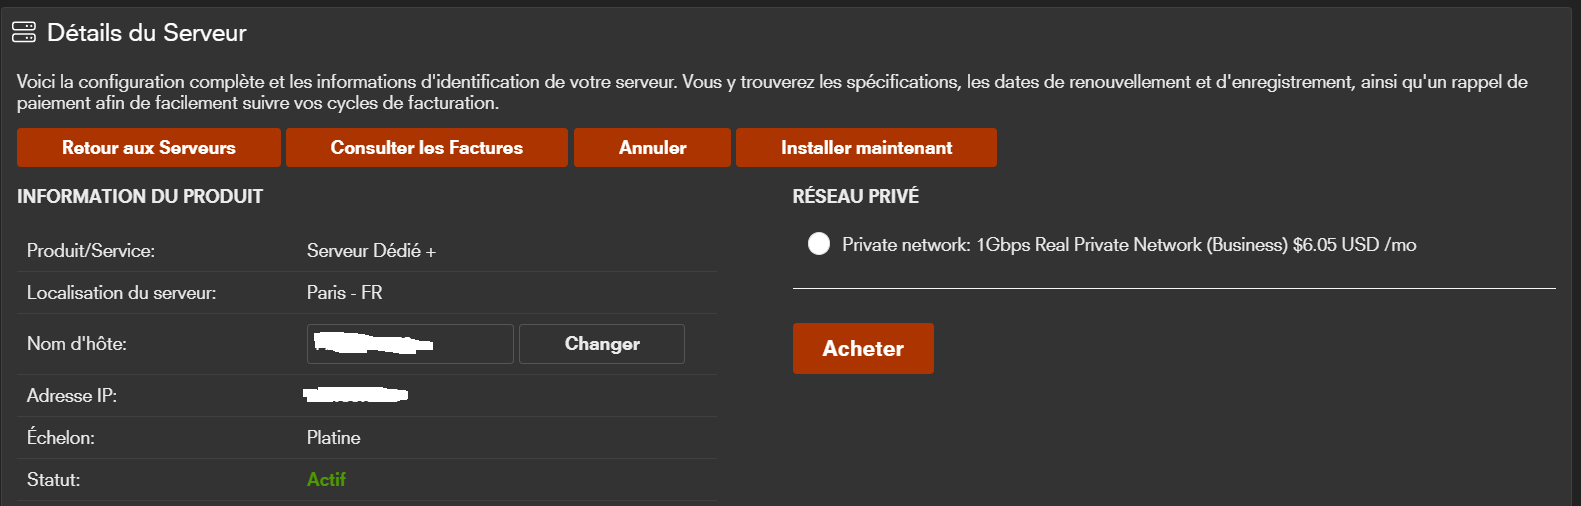
\includegraphics[width=0.9\textwidth]{figures/captures/dep_serveur_details.png}
    \caption{Fiche du serveur dans le panneau OneProvider}
    \label{fig:dep_serveur_details}
\end{figure}

\begin{figure}[H]
    \centering
    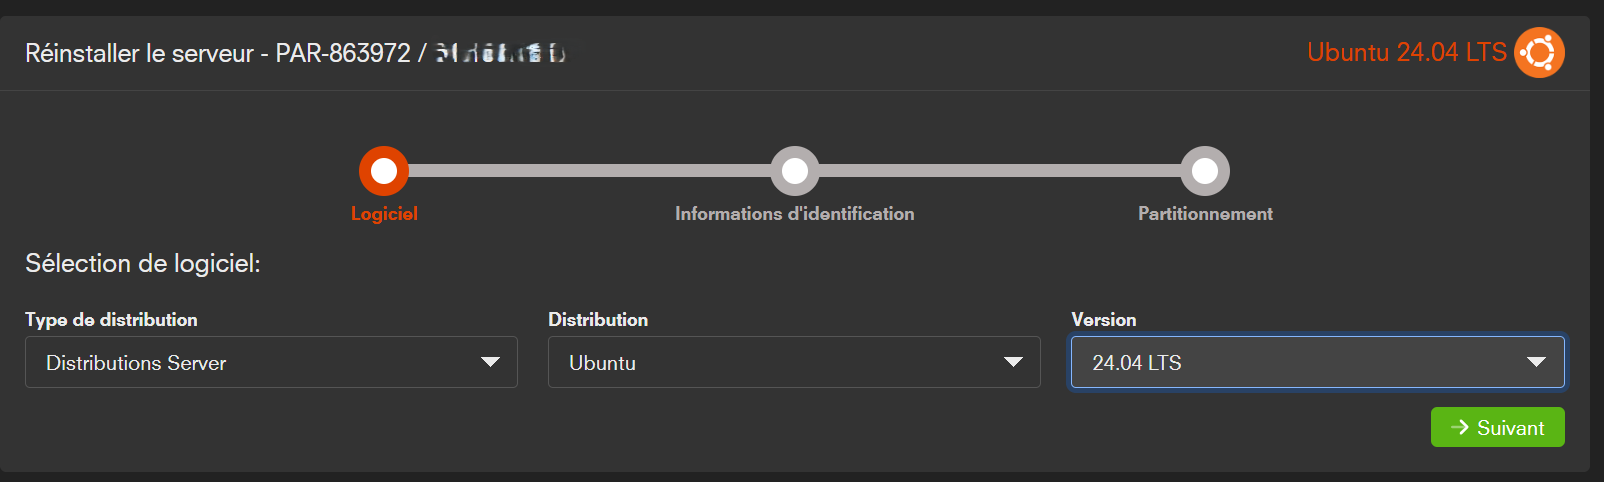
\includegraphics[width=0.9\textwidth]{figures/captures/dep_install_os.png}
    \caption{Réinstallation du serveur, étape 1 : choix d'Ubuntu 24.04 LTS}
    \label{fig:dep_install_os}
\end{figure}

\begin{figure}[H]
    \centering
    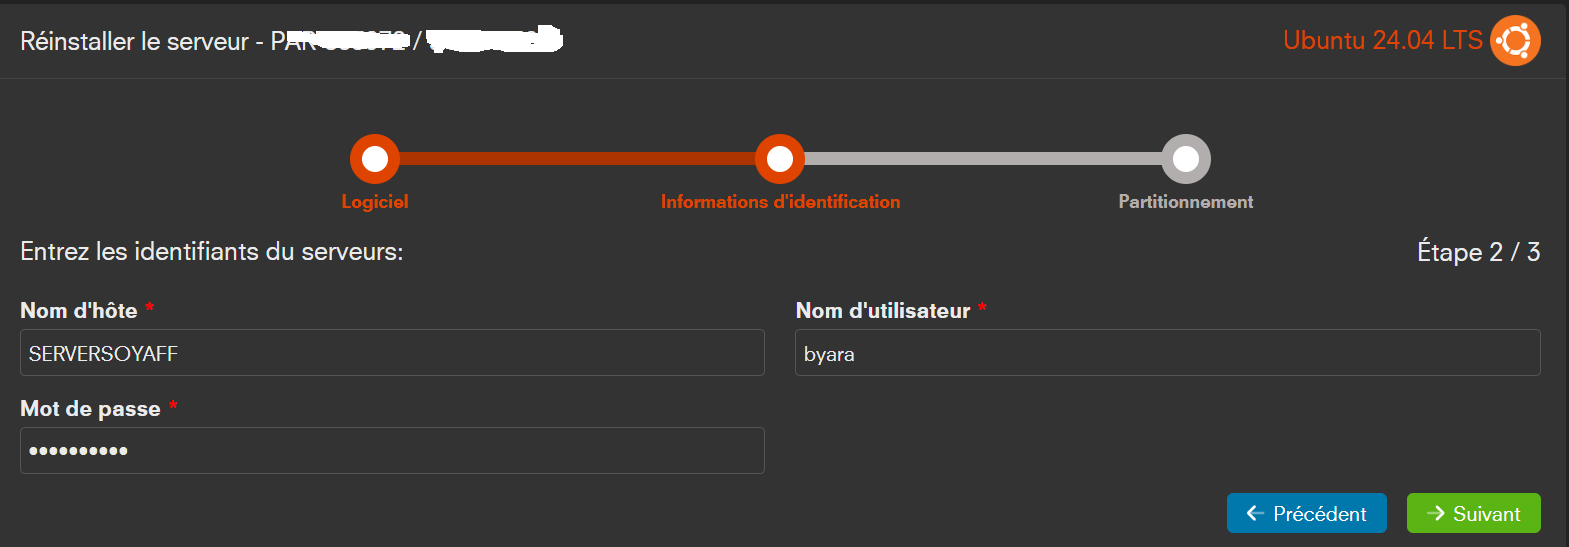
\includegraphics[width=0.9\textwidth]{figures/captures/dep_install_id.png}
    \caption{Réinstallation du serveur, étape 2 : nom d'hôte et compte d'administration}
    \label{fig:dep_install_id}
\end{figure}

\section{Préparation du système}

Après installation, le système a été mis à jour, le pare-feu configuré (Figure~\ref{fig:ops_ufw}), puis Docker installé par le script officiel. Le service Docker est configuré pour attendre le montage du disque qui porte ses données.

\begin{figure}[H]
    \centering
    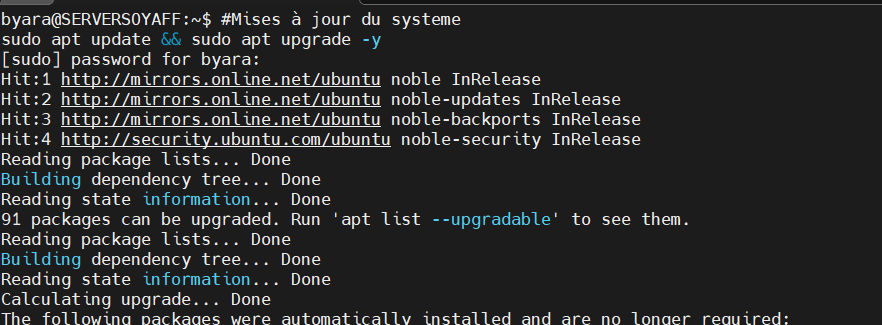
\includegraphics[width=0.8\textwidth]{figures/captures/dep_apt.png}
    \caption{Mise à jour du système}
    \label{fig:dep_apt}
\end{figure}

\begin{figure}[H]
    \centering
    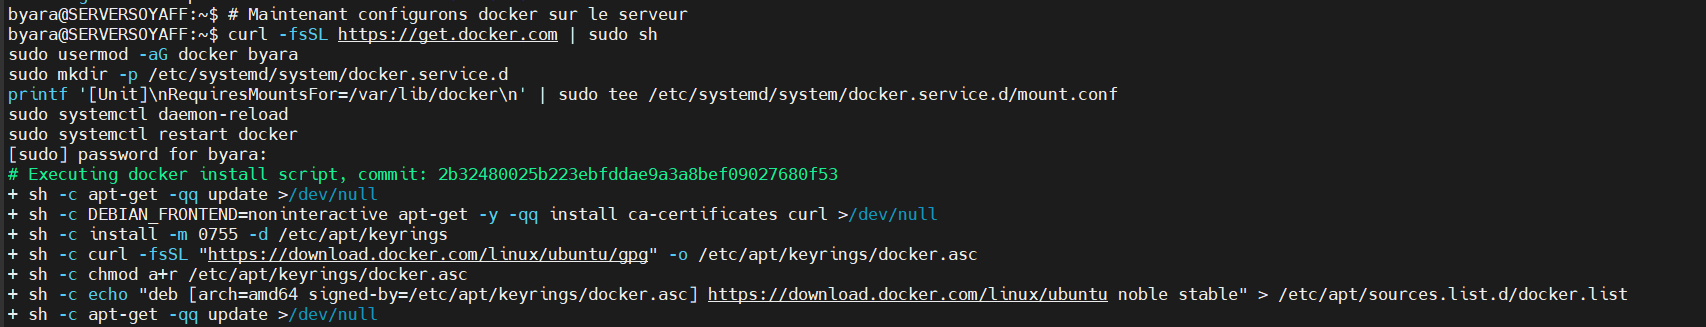
\includegraphics[width=\textwidth]{figures/captures/dep_docker.png}
    \caption{Installation de Docker et dépendance au montage de \texttt{/var/lib/docker}}
    \label{fig:dep_docker}
\end{figure}

\section{Déploiement de la pile IA/ETL}

Le pipeline de \texttt{assistant-soyaff} déploie la pile IA/ETL sur le serveur (\S\ref{sec:devops_cicd}). La Figure~\ref{fig:dep_deploy_ia_ps} montre l'état des conteneurs à l'issue d'un déploiement, et la Figure~\ref{fig:dep_arbo_detail} l'arborescence détaillée du dépôt sur le serveur.

\begin{figure}[H]
    \centering
    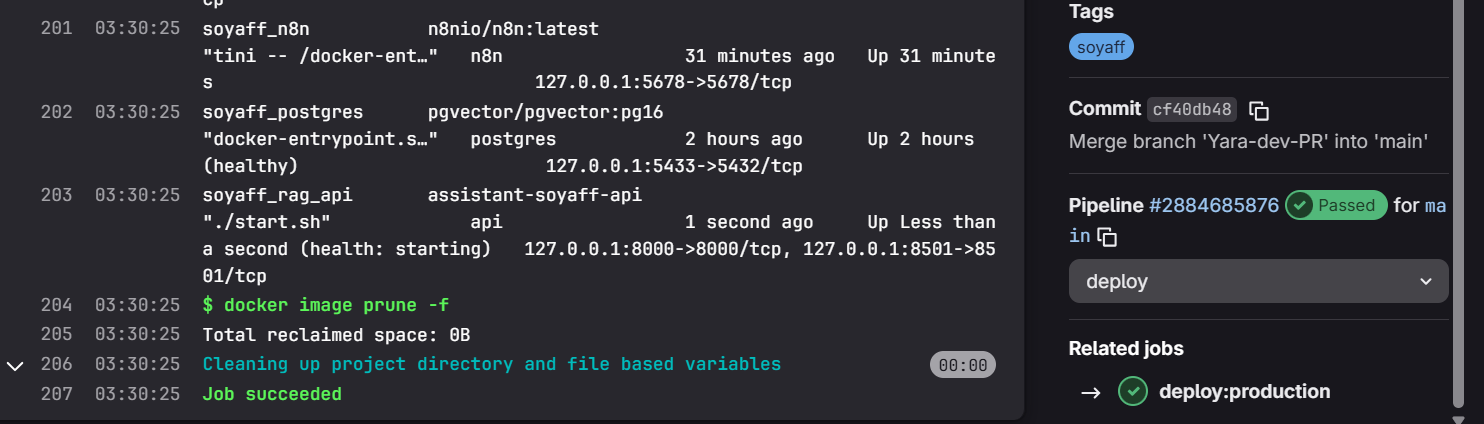
\includegraphics[width=0.85\textwidth]{figures/captures/dep_deploy_ia_ps.png}
    \caption{État des conteneurs de la pile IA/ETL en fin de déploiement}
    \label{fig:dep_deploy_ia_ps}
\end{figure}

\begin{figure}[H]
    \centering
    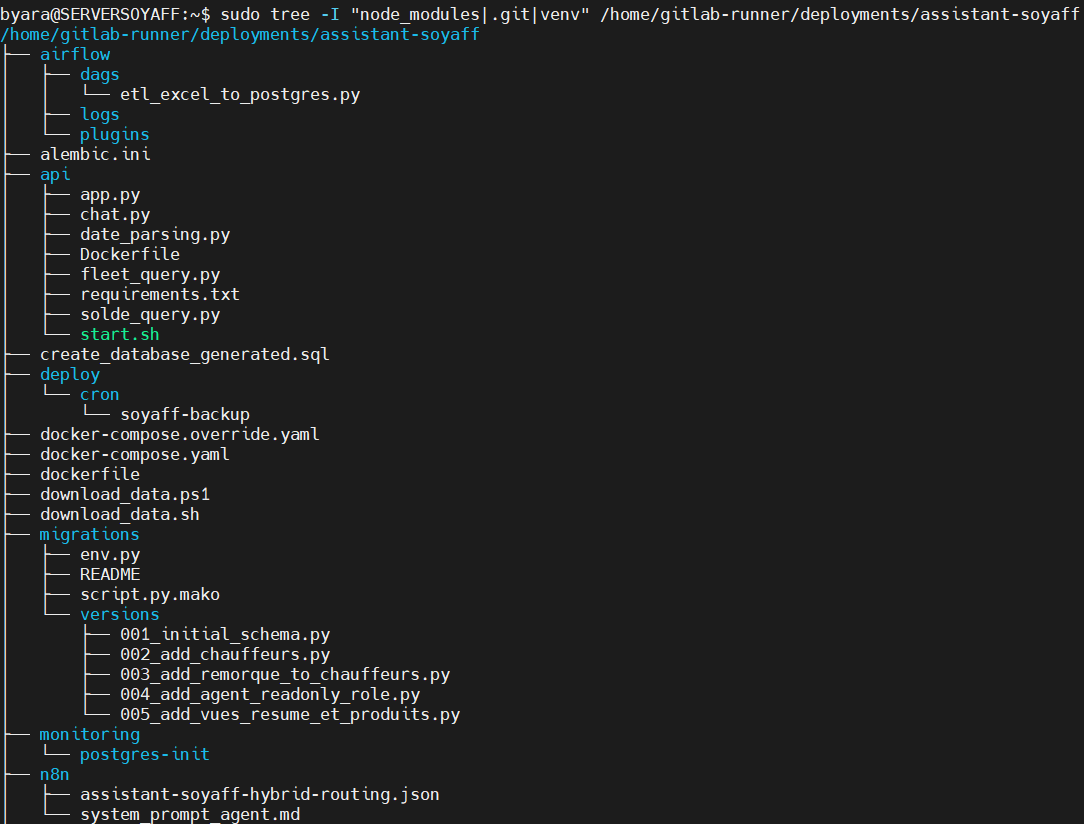
\includegraphics[width=0.75\textwidth]{figures/captures/dep_arbo_detail.png}
    \caption{Arborescence détaillée du dépôt \texttt{assistant-soyaff} sur le serveur}
    \label{fig:dep_arbo_detail}
\end{figure}

Les secrets (mots de passe de la base, clés d'API, jeton du bot Telegram) ne figurent dans aucun dépôt. Ils sont stockés dans les variables protégées de GitLab ; le job de déploiement génère le fichier \texttt{.env} du serveur à partir d'elles, à chaque exécution.

\section{Environnement de développement}

Avant chaque fusion sur \texttt{main}, les services sont exécutés sur le poste de développement avec les mêmes fichiers \texttt{docker compose} qu'en production (Figure~\ref{fig:dep_dev_local}).

\begin{figure}[H]
    \centering
    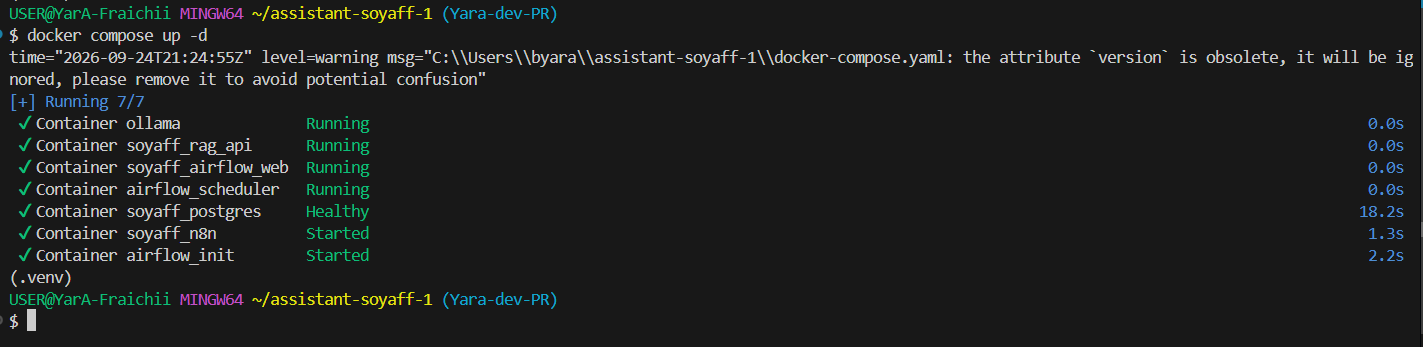
\includegraphics[width=\textwidth]{figures/captures/dep_dev_local.png}
    \caption{Démarrage de la pile IA/ETL sur le poste de développement}
    \label{fig:dep_dev_local}
\end{figure}

\section{Relevé des versions}

Les versions du Tableau~\ref{tab:env_versions} ont été relevées sur le serveur par les commandes suivantes.

\begin{lstlisting}[language=bash, basicstyle=\ttfamily\footnotesize, breaklines=true, showstringspaces=false]
lsb_release -ds; lscpu | grep -E "Model name|^CPU\(s\)"; free -h; df -h /
docker --version; docker compose version
docker exec soyaff_rag_api python --version
docker exec soyaff_postgres psql -U "$POSTGRES_USER" -d "$POSTGRES_DB" \
  -tAc "SELECT version();" \
  -tAc "SELECT extversion FROM pg_extension WHERE extname='vector';"
docker exec airflow_scheduler airflow version
docker exec ollama ollama --version; docker exec ollama ollama list
docker exec soyaff_n8n n8n --version
docker exec soyaff_backend node --version
\end{lstlisting}

\section{Sauvegarde planifiée}

\begin{sloppypar}
La sauvegarde (\S\ref{sec:devops_securite}) est déclarée dans le fichier versionné \texttt{deploy/cron/soyaff-backup}, installé dans \texttt{/etc/cron.d/}. Ses deux tâches actives sont les suivantes.
\end{sloppypar}

\begin{lstlisting}[basicstyle=\ttfamily\footnotesize, breaklines=true, showstringspaces=false]
# Sauvegarde quotidienne a 02:30 (archive locale + copie hors site)
30 2 * * * gitlab-runner cd $DEPLOY_PATH && scripts/backup_db.sh >> /var/log/soyaff/backup.log 2>&1
# Restauration d'essai chaque dimanche a 04:00, dans une base jetable
0 4 * * 0 gitlab-runner cd $DEPLOY_PATH && scripts/restore_db.sh --latest --drop-after >> /var/log/soyaff/restore-drill.log 2>&1
\end{lstlisting}
